\documentclass[11pt]{standalone}
\usepackage{amssymb}
\usepackage{amsmath}
\usepackage[no-math]{fontspec}
\usepackage{unicode-math}
\usepackage{libertinus}
\usepackage{pgf,xcolor}
\usepackage{tikz}
\usetikzlibrary{arrows.meta, backgrounds, calc}
\usepackage{pgfplots}
\pgfplotsset{compat=newest}

\definecolor{my_darkgray}{HTML}{484949}
\definecolor{my_lightgray}{HTML}{F3F4F4}
\definecolor{my_darkblue}{HTML}{005A94}
\definecolor{my_lightblue}{HTML}{CCDEE9}
\definecolor{my_yellow}{HTML}{FFEC7F}
\definecolor{my_red}{HTML}{E60000}
\definecolor{my_orange}{HTML}{E87846}

\begin{document}
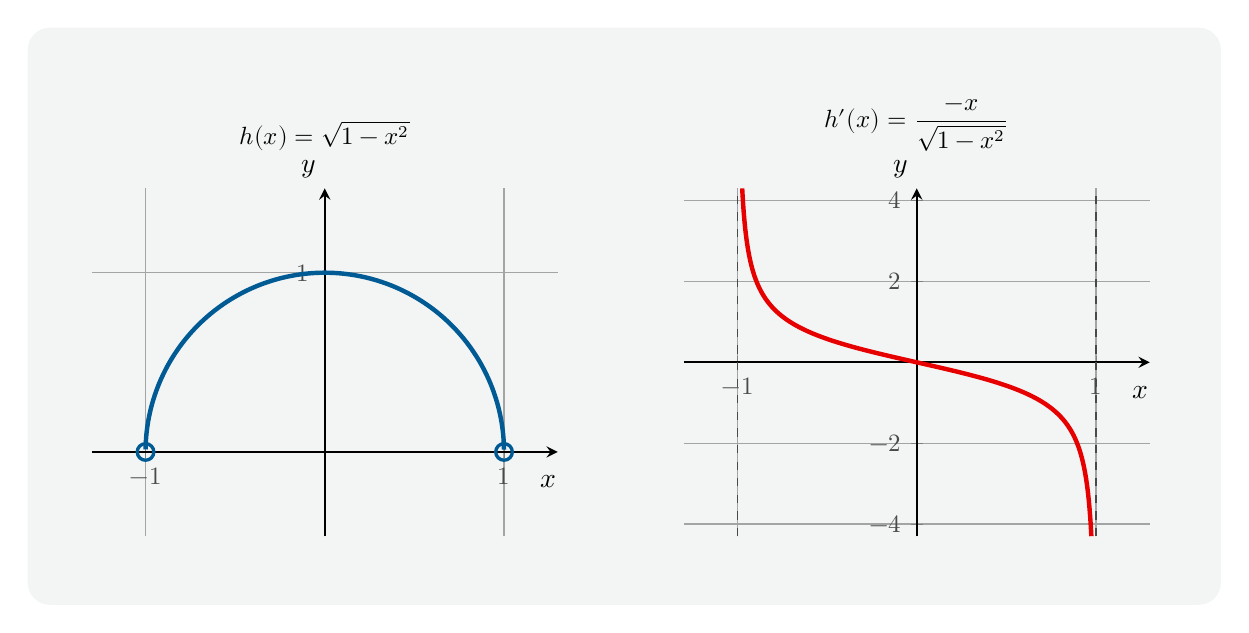
\begin{tikzpicture}[
    show background rectangle,
    background rectangle/.style={fill=my_lightgray, rounded corners=8pt},
    inner frame sep=0.8cm
]

% ── Left plot: h(x) = sqrt(1 - x²) ────────────────────────────────────────
% h is defined only on [-1, 1]; range is [0, 1].
% axis equal is used here: h traces the upper unit semicircle and equal
% scaling preserves its circular shape correctly.
\begin{axis}[
    name=left plot,
    axis lines = center,
    xlabel = {$x$},
    ylabel = {$y$},
    xlabel style = {at={(axis cs:1.25,0)}, anchor=north, yshift=-5pt},
    ylabel style = {anchor=south east},
    title = {$h(x) = \sqrt{1-x^2}$},
    title style = {font=\small, text=black, yshift=4pt},
    grid = both,
    grid style = {line width=0.3pt, draw=my_darkgray!30},
    major grid style = {line width=0.5pt, draw=my_darkgray!50},
    axis equal,
    axis line style = {thick},
    xmin = -1.3, xmax = 1.3,
    ymin = -0.3, ymax = 1.3,
    xtick = {-1, 0, 1},
    ytick = {0, 1},
    yticklabel style = {
        /pgf/number format/fixed,
        /pgf/number format/precision=0,
        font=\small,
        text=my_darkgray
    },
    xticklabel style = {font=\small, text=my_darkgray},
    width=7.5cm, height=6cm,
    clip=true,
]
% Domain kept strictly inside (-1, 1) to avoid sqrt(0) at the endpoints.
% restrict y to domain acts as a safety net against any residual artifacts.
\addplot[
    draw=my_darkblue,
    samples=800,
    ultra thick,
    domain=-0.9999:0.9999,
    restrict y to domain=0:1.5
]{ sqrt(1 - x^2) };

% Mark the open domain boundary at x = ±1, h(±1) = 0
\addplot[
    mark=o,
    mark size=3pt,
    only marks,
    draw=my_darkblue,
    fill=my_lightgray,
    line width=1.2pt
] coordinates {(-1, 0) (1, 0)};
\end{axis}

% ── Right plot: h'(x) = -x / sqrt(1 - x²) ─────────────────────────────────
% h' diverges as x → ±1; the plot is clipped to y ∈ [-4, 4].
% Domain is kept away from ±1 to avoid numerical blow-up; restrict y to
% domain provides an additional safety net at the clip boundary.
\begin{axis}[
    name=right plot,
    at={($(left plot.east)+(1.6cm,0)$)},
    anchor=west,
    axis lines = center,
    xlabel = {$x$},
    ylabel = {$y$},
    xlabel style = {at={(axis cs:1.25,0)}, anchor=north, yshift=-5pt},
    ylabel style = {anchor=south east},
    title = {$h'(x) = \dfrac{-x}{\sqrt{1-x^2}}$},
    title style = {font=\small, text=black, yshift=4pt},
    grid = both,
    grid style = {line width=0.3pt, draw=my_darkgray!30},
    major grid style = {line width=0.5pt, draw=my_darkgray!50},
    % axis equal omitted: y range ±4 vs x range ±1 would make the curve
    % appear as a nearly flat horizontal line
    axis line style = {thick},
    xmin = -1.3, xmax = 1.3,
    ymin = -4.3, ymax = 4.3,
    xtick = {-1, 0, 1},
    ytick = {-4, -2, 0, 2, 4},
    yticklabel style = {
        /pgf/number format/fixed,
        /pgf/number format/precision=0,
        font=\small,
        text=my_darkgray
    },
    xticklabel style = {font=\small, text=my_darkgray},
    width=7.5cm, height=6cm,
    clip=true,
]
\addplot[
    draw=my_red,
    samples=800,
    ultra thick,
    domain=-0.9990:0.9990,
    restrict y to domain=-4.5:4.5
]{ -x / sqrt(1 - x^2) };

% Mark the vertical asymptotes at x = ±1 with dashed lines
\addplot[
    draw=my_darkgray,
    dashed,
    thin,
    domain=-4.3:4.3
] coordinates {(-1,-4.3) (-1,4.3)};
\addplot[
    draw=my_darkgray,
    dashed,
    thin,
    domain=-4.3:4.3
] coordinates {(1,-4.3) (1,4.3)};

% Labels for the asymptotes
\node[anchor=south, font=\small, text=my_darkgray]
    at (axis cs:-1, 4.3) {$x=-1$};
\node[anchor=south, font=\small, text=my_darkgray]
    at (axis cs: 1, 4.3) {$x=1$};
\end{axis}

\end{tikzpicture}
\end{document}
